\chapter{高等数学}
	高等数学是硕士研究生招生考试考查内容之一,主要考查考生对高等数学的基本概念、基本理论、基本方法的理解和掌握以及考生的抽象思维能力、逻辑推理能力、综合运用能力和解决实际问题的能力。在考研数学一试卷中分值为82分,约占56\%。
		\section{极限、连续}
	\subsection{函数极限}
	\begin{ti}
		求 $\lim_{x\to 0} \frac{\sqrt{1+x} - 1 - \frac{x}{2}}{\ee^{x^{2}}-1}$.
	\end{ti}

	\begin{ti}
		求 $\lim_{x \to 0} \frac{\ee^{x} + \ln(1 - x) - 1}{x - \arctan x}$.
	\end{ti}

	\begin{ti}
		求 $\lim_{x \to 0} \frac{(1+x)^{\frac{2}{x}} - \ee^{2}[1 - \ln(1+x)]}{x}$.
	\end{ti}

	\begin{ti}
		求 $\lim_{x \to 0} \frac{\left(1 + x^{2}\right)(1 - \cos 2x) - 2x^{2}}{x^{4}}$.
	\end{ti}

	\begin{ti}
		求 $\lim_{x \to 0} \frac{\sqrt{1-x^{2}} \sin^{2}x - \tan^{2}x }{x^{2}[\ln(1+x)]^{2}}$.
	\end{ti}

	\begin{ti}
		求 $\lim_{x \to 0} \frac{(3 + 2 \tan x)^{x} - 3^{x}}{3 \sin^{2}x + x^{3} \cos\frac{1}{x}}$.
	\end{ti}

	\begin{ti}
		求 $\lim_{x \to 2}\frac{\sqrt{5x - 1} - \sqrt{2x + 5}}{x^{2} - 4}$.
	\end{ti}

	\begin{ti}
		求 $\lim_{x \to 0}\int_{0}^{x} \frac{\sin 2t}{\sqrt{4+t^{2}}\int_{0}^{x} \left(\sqrt{t+1} - 1\right)\dd{t}} \dd{t}$.
	\end{ti}

	\begin{ti}
		求 $\lim_{x \to \infty} \ee^{-x} \left( 1 + \frac{1}{x} \right)^{x^{2}}$.
	\end{ti}

	\begin{ti}
		求 $\lim_{x \to 3^{+}} \frac{\cos x \ln (x - 3)}{\ln\left( \ee^{x} - \ee^{3} \right)}$.
	\end{ti}

	\begin{ti}
		求 $\lim_{x \to \infty} x^{2} \left( a^{\frac{1}{x}} + a^{-\frac{1}{x}} - 2 \right)$,其中常数 $a > 0$.
	\end{ti}

	\begin{ti}
		求 $\lim_{x \to 0}\frac{1}{x}\left( \cot x - \frac{1}{x} \right)$.
	\end{ti}

	\begin{ti}
		求 $\lim_{x \to +\infty}\left( \sqrt[3]{x^{3} + 2x^{2} + 1} - x\ee^{\frac{1}{x}} \right)$.
	\end{ti}

	\begin{ti}
		求 $\lim_{x \to 0}\left( \frac{1+x}{1-e^{-x}} - \frac{1}{x} \right)$.
	\end{ti}

	\begin{ti}
		求 $\lim_{x \to 0^{+}} x^{\ln\left( \frac{\ln x - 1}{\ln x + 1} \right)}$.
	\end{ti}

	\begin{ti}
		求 $\lim_{x \to \infty} \left( \tan\frac{\uppi x}{1 + 2x} \right)^{\frac{1}{x}}$.
	\end{ti}

	\begin{ti}
		求 $\lim_{x \to 0^{+}} \left( \frac{\sin x}{x} \right)^{\frac{1}{1 - \cos x}}$.
	\end{ti}

	\begin{ti}
		求 $\lim_{x \to 0}\left( \frac{\cos x}{\cos 2x} \right)^{\frac{1}{x^{2}}}$.
	\end{ti}

	\begin{ti}
		求 $\lim_{x \to 0} \frac{\sin x - x\cos x}{x - \sin x}$.
	\end{ti}

	\begin{ti}
		求 $\lim_{x \to 0}\frac{1 + \frac{1}{2}x^{2} - \sqrt{1 + x^{2}}}{\left( \cos x - \ee^{\frac{x^{2}}{2}} \right) \sin \frac{x^{2}}{2}}$.
	\end{ti}

	\begin{ti}
		求 $\lim_{x \to \infty} \left( \sqrt[6]{x^{6} + x^{5}} - \sqrt[6]{x^{6} - x^{5}} \right)$.
	\end{ti}

	\begin{ti}
		求 $\lim_{x \to +\infty}\left[ \left( x^{3} + \frac{x}{2} - \tan \frac{1}{x} \right) \ee^{\frac{1}{x}} - \sqrt{1 + x^{6}} \right]$.
	\end{ti}

	\begin{ti}
		求 $\lim_{x \to 0}\frac{\ee^{\tan x} - \ee^{\sin x}}{x \sin^{2} x}$.
	\end{ti}

	\begin{ti}
		求 $\lim_{x \to 0} \frac{\sin x + x^{2} \sin\frac{1}{x}}{(1 + \cos x)\ln(1 + x)}$.
	\end{ti}

	\begin{ti}
		求 $\lim_{x \to 0}\left[ \frac{a}{x} - \left( \frac{1}{x^{2}} - a^{2} \right) \ln(1 + ax) \right]$,其中 $a \ne 0$.
	\end{ti}

	\begin{ti}
		求 $\lim_{x \to 0} \frac{(1 + x)^{\frac{1}{x}} - (1 + 2x)^{\frac{1}{2x}}}{\sin x}$.
	\end{ti}

	\begin{ti}
		求 $\lim_{x \to 0}\frac{\int_{0}^{\sin^{2}x} \ln(1 + t)\dd{t}}{\left( \sqrt[3]{1 + x^{3}} - 1 \right)\sin x}$.
	\end{ti}

	\begin{ti}
		求 $\lim_{x \to 0} \frac{ \int_{0}^{x} \left[ \int_{0}^{u^{2}} \arctan(1 + t) \dd{t} \right] \dd{u} }{x(1 - \cos x)}$.
	\end{ti}

	\begin{ti}
		求 $\lim_{x \to 0^{+}} \frac{x^{x} - ( \sin x )^{x}}{x^{2}\ln(1 + x)}$.
	\end{ti}

	\begin{ti}
		求 $\lim_{x \to 0} \frac{ \cos x - \ee^{-\frac{x^{2}}{2}} }{x^{2} [ x + \ln(1 - x) ]}$.
	\end{ti}

	\begin{ti}
		求 $\lim_{x \to 0} \frac{1}{x^{3}} \left[ \left( \frac{2 + \cos x}{3} \right)^{x} - 1 \right]$.
	\end{ti}

	\begin{ti}
		求 $\lim_{x \to 0} \frac{\ln\left( \sin^{2}x + \ee^{x} \right) - x}{\ln\left( x^{2} + \ee^{2x} \right) - 2x}$.
	\end{ti}

	\begin{ti}
		求 $\lim_{x \to 1} \frac{x - x^{x}}{1 - x + \ln x}$.
	\end{ti}

	\begin{ti}
		求 $\lim_{x \to 0} \left( \frac{a_{1}^{x} + a_{2}^{x} + \cdots + a_{n}^{x}}{n} \right)^{\frac{1}{x}}$,$a_{i} > 0$,且 $a_{i} \ne 1, i = 1,2,\cdots,n,n \geq 2$.
	\end{ti}

	\begin{ti}
		设 $\lim_{x \to 0} \frac{\ln\left[ 1 + \frac{f(x)}{\sin x} \right]}{a^{x} - 1} = A (a > 0, a \ne 1)$,求 $\lim_{x \to 0}\frac{f(x)}{x^{2}}$.
	\end{ti}

	\begin{ti}
		已知 $\lim_{x \to 1} f(x)$ 存在,且 $f(x) = \frac{x - \arctan(x - 1) - 1}{(x - 1)^{3}} + 2x^{2} \ee^{x-1} \cdot \lim_{x \to 1} f(x)$,求 $f(x)$.
	\end{ti}

	\begin{ti}
		设函数 $f(x) = (1 + x)^{\frac{1}{x}}(x > 0)$,证明:存在常数 $A,B$,使得当 $x \to 0^{+}$ 时,恒有
		\begin{equation*}
			f(x) = \ee + Ax +Bx^{2} + o\left( x^{2} \right),
		\end{equation*}
		并求常数 $A,B$.
	\end{ti}

	\begin{ti}
		已知 $\lim_{x \to 0} \frac{(1+x)^{\frac{1}{x}} - \left( A + Bx + Cx^{2} \right)}{x^{3}} = D \ne 0$. 求常数 $A,B,C,D$.
	\end{ti}

	\begin{ti}
		设函数 $f(x) = \begin{cases}
			\frac{\ln\left( 1 + x^{3} \right)}{\arcsin x - x}, & x < 0,\\
			\frac{\ee^{-x} + \frac{1}{2}x^{2} + x - 1}{x \sin \frac{x}{6}}, & x > 0,
		\end{cases}$,$g(x) = \frac{\ee^{\frac{1}{x}}\arctan\frac{1}{x}}{1 + \ee^{\frac{2}{x}}}$,求 $\lim_{x \to 0} f[g(x)]$.
	\end{ti}

	\begin{ti}
		设 $\alpha \geq 5$ 且为常数,则 $k$ 为何值时极限
		\begin{equation*}
			I = \lim_{x \to +\infty} \left[ \left( x^{\alpha} + 8x^{4} + 2 \right)^{k} - x \right]
		\end{equation*}
		存在,并求此极限值.
	\end{ti}
	
	\begin{ti}
		已知极限
		\[
			I = \lim_{x \to 0} \left( \frac{a}{x^{2}} + \frac{b}{x^{4}} + \frac{c}{x^{5}} \int_{0}^{x} \ee^{-t^{2}} \dd{t} \right) = 1,
		\]
		求常数 $a,b,c$.
	\end{ti}

	\begin{ti}
		求 $\lim_{x \to 0} \frac{ \sqrt{\cos x} - \sqrt[3]{\cos x} }{\sin^{2}x}$.
	\end{ti}

	\begin{ti}
		求 $\lim_{x \to 1} \frac{\left( 1 - \sqrt[3]{x} \right) \left( 1 - \sqrt[4]{x} \right) \cdots \left( 1 - \sqrt[n]{x} \right) }{(1 - x)^{n-2}}$.
	\end{ti}
	
	\begin{ti}
		求 $\lim_{x \to 0} \frac{1 - \cos x \cdot \sqrt{\cos 2x} \cdot \sqrt[3]{\cos 3x}}{x^{2}}$.
	\end{ti}

	\begin{ti}
		设函数 $f(x)$ 满足 $f(1) = 1$,且有 $f'(x) = \frac{1}{x^{2} + f^{2}(x)}$,证明:极限 $\lim_{x \to \infty} f(x)$ 存在,且极限值小于 $1 + \frac{\uppi}{4}$.
	\end{ti}

	\begin{ti}
		设 $x \geq 0$ 时,$f(x)$ 满足 $f'(x) = \frac{1}{x^{2} + f^{2}(x)}$,且 $f(0) = 1$,证明:$\lim_{x \to +\infty} f(x)$ 存在且极限值小于 $1 + \frac{\uppi}{2}$.
	\end{ti}
	\subsection{无穷小比阶}

	\begin{ti}
		当 $x \to 0$ ,$(1 - \cos x)\ln\left( 1 + 2x^{3} \right)$ 是比 $x \sin x^{n}$ 高阶的无穷小,而 $x \sin x^{n}$ 是比 $\ee^{x\tan^{2} x} - 1$ 高阶的无穷小,则正整数 $n = $ \htwo.
	\end{ti}

	\begin{ti}
		当 $x \to 0^{+}$ 时,$\sqrt{1 + \tan \sqrt{x}} - \sqrt{1 + \sin\sqrt{x}}$ 是 $x$ 的 $k$ 阶无穷小,则 $k =$ \htwo.
	\end{ti}

	\begin{ti}
		当 $x \to 0$ 时,$f(x) = \ln\left( 1+x^{2} \right) - 2\sqrt[3]{\left( \ee^{x} - 1 \right)^{2}}$ 是无穷小量 $x^{k}$ 的同阶无穷小,则 $k = $ \kuo.

		\fourch{$1$}{$2$}{$\frac{2}{3}$}{$\frac{3}{2}$}
	\end{ti}

	\begin{ti}
		当 $x \to 0$ 时,下列无穷小量中,最高阶的无穷小是\kuo.

		\twoch{$\ln\left( x + \sqrt{1 + x^{2}} \right)$}{$1 - \cos x$}{$\tan x - \sin x$}{$\ee^{x} + \ee^{-x} - 2$}
	\end{ti}

	\begin{ti}
		当 $x \to 0^{+}$ 时,下列无穷小量中,与 $x$ 同阶的无穷小是\kuo.

		\twoch{$\sqrt{1 + x} - 1$}{$\ln(1 + x) - x$}{$\cos(\sin x) - 1$}{$x^{x} - 1$}
	\end{ti}

	\begin{ti}
		当 $x \to 0$ 时,$f(x) = x - \sin x + \int_{0}^{x} t^{2} \ee^{t^{2}} \dd{t}$ 是 $x$ 的 $k$ 阶无穷小,则 $k=$ \kuo.

		\fourch{$3$}{$4$}{$5$}{$6$}
	\end{ti}

	\begin{ti}
		当 $x \to 0^{+}$ 时,试比较无穷小量 $\alpha$,$\beta$ 和 $\gamma$ 三者之间的阶,其中
		\[
			\alpha = \int_{0}^{x} \cos t^{2} \dd{t},\beta = \int_{0}^{x^{2}} \tan \sqrt{t} \dd{t},\gamma = \int_{0}^{\sqrt{x}} \sin t^{3} \dd{t}.
		\]
	\end{ti}

	\begin{ti}
		当 $x \to 0$ 时,$\sin x \left( \cos x - 4 \right) + 3x$ 为 $x$ 的几阶无穷小?
	\end{ti}

	\begin{ti}
		当 $x \to 0$ 时,确定下列无穷小量的阶数:
		\begin{enumerate}
			\item $\tan\left( \sqrt{x+2} - \sqrt{2} \right)$;
			\item $\sqrt[3]{1 + \sqrt[3]{x}} - 1$;
			\item $3^{\sqrt{x}} - 1$.  
		\end{enumerate}
	\end{ti}

	\begin{ti}
		当 $x \to 0$ 时,$x - \sin x \cos x \cos 2x$ 与 $cx^{k}$ 为等价无穷小,则 $c=$ \htwo,$k=$ \htwo.
	\end{ti}

	\begin{ti}
		当 $x \to 0$ 时,$1 - \cos x \cos 2x \cos 3x$ 对于无穷小 $x$ 的阶数等于 \htwo.
	\end{ti}

	\begin{ti}
		极限 $\lim_{x \to \infty} \frac{\ee^{\sin\frac{1}{x}}-1}{\left( 1 + \frac{1}{x} \right)^{\alpha} - \left( 1 + \frac{1}{x} \right)} = A \ne 0$ 的充要条件是 \kuo.

		\twoch{$\alpha > 1$}{$\alpha \ne 1$}{$\alpha > 0$}{与 $\alpha$ 无关}
	\end{ti}

	\begin{ti}
		设当 $x \to 0$ 时,$\ee^{\tan x} - \ee^{x}$ 与 $x^{n}$ 是同阶无穷小,则 $n$ 为 \kuo.

		\fourch{$1$}{$2$}{$3$}{$4$}
	\end{ti}

	\begin{ti}
		设当 $x \to 0$ 时,$f(x) = ax^{3} + bx$ 与 $g(x) =$ $\int_{0}^{\sin x} \left( \ee^{t^{2}} -1 \right) \dd{t}$ 是等价无穷小,则\kuo.

		\twoch{$a = \frac{1}{3},b=1$}{$a = 3,b=0$}{$a = \frac{1}{3},b=0$}{$a = 1,b=0$}
	\end{ti}

	\begin{ti}
		设当 $x \to 0$ 时,$f(x) = \ln\left( 1+x^{2} \right) - \ln\left( 1 + \sin^{2}x \right)$ 是 $x$ 的 $n$ 阶无穷小,则正整数 $n$ 为\kuo.
		
		\fourch{$1$}{$2$}{$3$}{$4$}
	\end{ti}

	\begin{ti}
		当 $x \to \uppi$ 时,若有 $\sqrt[4]{\sin\frac{x}{2}} - 1 \sim A(x - \uppi)^{k}$,则 $A=$\htwo,$k=$\htwo.
	\end{ti}

	\begin{ti}
		半径分别为 $R,r(R>r>0)$ 的两个圆相切于坐标轴原点. 如图~\ref{fig:1.1.1} 所示.
		\begin{enumerate}
			\item 当 $x \to 0^{+}$ 时,若线段长 $MM_{1}$ 与 $x^{k}$ 同阶,求 $k$;
			\item 当 $x \to 0^{+}$ 时,若 $\angle MOM_{1}$ 与 $x^{c}$ 同阶,求 $c$.
		\end{enumerate}
		\begin{figure}[htbp]
			\centering
			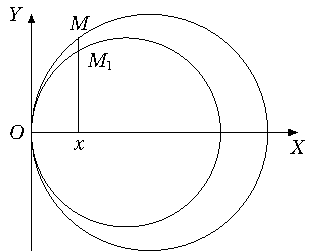
\includegraphics[scale=1]{figure/fig1-1-1.pdf}
			\caption{}\label{fig:1.1.1}
		\end{figure}
	\end{ti}
	\subsection{数列极限}

	\begin{ti}
		求 $\lim_{n \to \infty} n^{3} \left( \sin\frac{1}{n} - \frac{1}{2} \sin\frac{2}{n} \right)$.
	\end{ti}

	\begin{ti}
		求 $\lim_{n \to \infty} \left( \sqrt{n + 3\sqrt{n}} - \sqrt{n - \sqrt{n}} \right)$.
	\end{ti}

	\begin{ti}
		求 $\lim_{n \to \infty} \left[ \sqrt{n}\left( \sqrt{n+1} - \sqrt{n} \right) + \frac{1}{2} \right]^{\frac{\sqrt{n+1} + \sqrt{n}}{\sqrt{n+1} - \sqrt{n}}}$.
	\end{ti}

	\begin{ti}
		求 $\lim_{n \to \infty} n^{2} \left( a^{\frac{1}{n}} - a^{\frac{1}{n+1}} \right)$,其中 $a > 0$.
	\end{ti}

	\begin{ti}
		求 $\lim_{n \to \infty} \left( 1 + 2^{n} + 3^{n} \right)^{\frac{1}{n}}$.
	\end{ti}

	\begin{ti}
		求 $\lim_{n \to \infty} \cos\frac{x}{2}\cos\frac{x}{4}\cdots \cos\frac{x}{2^{n}}$.
	\end{ti}

	\begin{ti}
		求 $\lim_{n \to \infty} n^{2}\left( \arctan\frac{a}{n} - \arctan \frac{a}{n+1} \right)$,$a > 0$.
	\end{ti}

	\begin{ti}
		设 $\lim_{n \to \infty} \frac{n^{99}}{n^{k} - (n-1)^{k}}$ 存在且不为零,则常数 $k =$
		
		\noindent\hone{2}.
	\end{ti}

	\begin{ti}
		设数列 $\{ a_{n} \}$ 满足 $\lim_{n \to \infty}\frac{a_{n+1}}{a_{n}} = 1$,则\kuo.

		\twoch{$\{ a_{n} \}$ 有界}{$\{ a_{n} \}$ 不存在极限}{$\{ a_{n} \}$ 自某项起同号}{$\{ a_{n} \}$ 自某项起单调}
	\end{ti}

	\begin{ti}
		设数列 $\{ x_{n} \}$ 满足 $x_{n} > 0$,且 $\lim_{n \to \infty}\frac{x_{n+1}}{x_{n}} = \frac{1}{2}$,则\kuo.

		\onech{$\lim_{n\to\infty}x_{n} = 0$}{$\lim_{n\to\infty}x_{n}$ 存在,但不为零}{$\lim_{n\to\infty}x_{n}$ 不存在}{$\lim_{n\to\infty}x_{n}$ 可能存在,也可能不存在}
	\end{ti}

	\begin{ti}
		已知数列 $\{ a_{n} \}$ 单调,下列结论正确的是\kuo.
		
		\twoch{$\lim_{n \to \infty}\left( \ee^{a_{n}} - 1 \right)$ 存在}{$\lim_{n \to \infty} \frac{1}{1 + a_{n}^{2}}$ 存在}{$\lim_{n \to \infty} \sin a_{n}$ 存在}{$\lim_{n \to \infty} \frac{1}{1 - a_{n}^{2}}$ 存在}
	\end{ti}

	\begin{ti}
		设 $a_{1} = 1$,$a_{2} = 2$,$a_{n+2} = \frac{2a_{n}a_{n+1}}{a_{n} + a_{n+1}} (n=1,2,\cdots)$.
		\begin{enumerate}
			\item 求 $b_{n} = \frac{1}{a_{n+1}} - \frac{1}{a_{n}}$ 的表达式;
			\item 求 $\sum_{k=1}^{n} b_{k}$ 和 $\lim_{n \to \infty} a_{n}$.
		\end{enumerate}
	\end{ti}

	\begin{ti}
		设 $a_{1} = 3$,$a_{n+1} = a_{n}^{2} + a_{n}(n = 1,2,\cdots)$,求极限
		\[
			\lim_{n \to \infty} \left( \frac{1}{1 + a_{1}} + \frac{1}{1 + a_{2}} + \cdots + \frac{1}{1 + a_{n}} \right).
		\]
	\end{ti}
	
	\begin{ti}
		已知 $x_{1} = \frac{1}{2}$,$2 x_{n+1} + x_{n}^{2} = 1$,求 $\lim_{n \to \infty} x_{n}$.
	\end{ti}

	\begin{ti}
		设 $x_{1} = 1$,$x_{n} = 1 + \frac{1}{1 + x_{n-1}}(n = 2,3,\cdots)$. 证明 $\lim_{n \to \infty} x_{n}$ 存在,并求该极限.
	\end{ti}

	\begin{ti}
		设 $x_{1} = 1$,$x_{n+1} = \frac{x_{n} + 3}{x_{n} + 1}$,求 $\lim_{n \to \infty} x_{n}$.
	\end{ti}

	\begin{ti}
		设当 $a \leq x \leq b$ 时,$a \leq f(x) \leq b$,并设存在常数 $k$,$0 \leq k < 1$,对于 $[a,b]$ 上的任意两点 $x_{1}$ 与 $x_{2}$,都有 $|f(x_{1}) - f(x_{2})| \leq k |x_{1} - x_{2}|$. 证明:
		\begin{enumerate}
			\item 存在唯一的 $\xi \in [a,b]$ 使 $f(\xi) = \xi$;
			\item 对于任意给定的 $x_{1} \in [a,b]$,定义 $x_{n+1} = f(x_{n})$,$n = 1,2,\cdots$,则 $\lim_{n \to \infty} x_{n}$ 存在,且 $\lim_{n \to \infty} x_{n} = \xi$.
		\end{enumerate}
	\end{ti}

	\begin{ti}
		已知 $\left( 2 + \sqrt{2} \right)^{n} = A_{n} + B_{n}\sqrt{2}$,$A_{n},B_{n}$ 为整数,$n = 1,2,3,\cdots$,求 $\lim_{n\to \infty} \frac{A_{n}}{B_{n}}$.
	\end{ti}

	\begin{ti}
		设 $f(x)$ 在 $[0,+\infty)$ 上连续,满足 $0 \leq f(x) \leq x, x \in [0,+\infty)$,设 $a_{1} \geq 0$,$a_{n+1} = f(a_{n})(n = 1,2,\cdots)$,证明:
		\begin{enumerate}
			\item $\{ a_{n} \}$ 为收敛数列;
			\item 设 $\lim_{n \to \infty} a_{n} = t$,则有 $f(t) = t$;
			\item 若条件改为 $0 \leq f(x) < x,x \in (0,+\infty)$,则 $t = 0$.
		\end{enumerate}
	\end{ti}

	\begin{ti}
		\begin{enumerate}
			\item 设 $f(x) = x + \ln(2 - x)$,求 $f(x)$ 的最大值;
			\item 设 $x_{1} = \ln 2$,$x_{n} = \sum_{i=1}^{n-1} \ln(2 - x_{i}), n = 2,3,\cdots$,证明 $\lim_{n \to \infty} x_{n}$ 存在并求其极限值.
		\end{enumerate}
	\end{ti}

	\begin{ti}
		设 $x_{1} = 1$,$x_{n} = \int_{0}^{1} \min\{x,x_{n-1}\} \dd{x}, n = 2,3,\cdots$,证明 $\lim_{n \to \infty} x_{n}$ 存在并求其极限值.
	\end{ti}

	\begin{ti}
		设数列 $\{ x_{n} \}$ 满足 $0 < x_{1} < 1$,$\ln(1 + x_{n}) = \ee^{x_{n+1}} - 1(n = 1,2,\cdots)$,证明
		\begin{enumerate}
			\item 当 $0 < x < 1$ 时,$\ln(1 + x) < x < \ee^{x} - 1$;
			\item $\lim_{n \to \infty} x_{n}$ 存在,并求该极限.
		\end{enumerate}
	\end{ti}

	\begin{ti}
		\begin{enumerate}
			\item 证明方程 $x = 2\ln(1 + x)$ 在 $(0,+\infty)$ 内有唯一实根 $\xi$;
			\item 任取 $x_{1} > \xi$,定义 $x_{n+1} = 2\ln(1 + x_{n}), n = 1,2,\cdots$,证明 $\lim_{n \to \infty} x_{n} = \xi$.
		\end{enumerate}
	\end{ti}

	\begin{ti}
		\begin{enumerate}
			\item 证明方程 $\ee^{x} + x^{2n+1} = 0$ 在 $(-1,0)$ 内有唯一实根 $x_{n}, n = 0,1,2,\cdots$;
			\item 证明 $\lim_{n \to \infty} x_{n}$ 存在并求其值 $a$;
			\item 求 $\lim_{n \to \infty} n(x_{n} - a)$.
		\end{enumerate}
	\end{ti}

	\begin{ti}
		设 $F(x,y) = \frac{f(y - x)}{2x}$,$F(1,y) = \frac{y^{2}}{2} - y + 5$,$x_{0} > 0$,$x_{1} = F(x_{0},2x_{0})$,$\cdots$,$x_{n+1} = F(x_{n},2x_{n}), n = 1,2,\cdots$. 证明 $\lim_{n \to \infty} x_{n}$ 存在,并求该极限.
	\end{ti}

	\begin{ti}
		已知
		\[
			f_{n}(x) = \CC_{n}^{1} \cos x - \CC_{n}^{2} \cos^{2}x + \cdots + (-1)^{n-1} \CC_{n}^{n} \cos^{n}x.
		\]
		\begin{enumerate}
			\item 证明方程 $f_{n}(x) = \frac{1}{2}$ 在区间 $\left( 0,\frac{\uppi}{2} \right)$ 中仅有一根 $x_{n}, n = 1,2,3,\cdots$;
			\item 求 $\lim_{n \to \infty} f_{n}\left( \arccos\frac{1}{n} \right)$;
			\item 设 $x_{n} \in \left( 0,\frac{\uppi}{2} \right)$ 满足 $f_{n}(x_{n}) = \frac{1}{2}$,证明 $\lim_{n \to \infty} x_{n} = \frac{\uppi}{2}$.
		\end{enumerate}
	\end{ti}

	\begin{ti}
		\begin{enumerate}
			\item 证明:当 $x \to 0^{+}$ 时,不等式 $0 < \tan^{2}x - x^{2} < x^{4}$ 成立;
			\item 设 $x_{n} = \sum_{k=1}^{n} \tan^{2}\frac{1}{\sqrt{n+k}}$,求 $\lim_{n \to \infty}x_{n}$.
		\end{enumerate}
	\end{ti}

	\begin{ti}
		\begin{enumerate}
			\item 设 $f(x)$ 在 $(0,+\infty)$ 内可导,$f'(x) > 0, x \in (0,+\infty)$,证明 $f(x)$ 在 $(0,+\infty)$ 内单调增加;
			\item 证明 $f(x) = \left( n^{x} + 1 \right)^{-\frac{1}{x}}$ 在 $(0,+\infty)$ 内单调增加,其中 $n$ 为正整数;
			\item 设数列 $x_{n} = \sum_{k=1}^{n} \left( n^{k} + 1 \right)^{-\frac{1}{k}}$,求 $\lim_{n \to \infty} x_{n}$.
		\end{enumerate}
	\end{ti}
	\subsection{连续与间断}

	\begin{ti}
		当 $x \in \left( -\frac{1}{2},1 \right]$ 时,确定函数 $f(x) = \frac{\tan \uppi x}{|x|\left( x^{2} - 1 \right)}$ 的间断点,并判定其类型.
	\end{ti}

	\begin{ti}
		确定函数 $f(x) = \frac{x(x - 1)}{|x| x^{2} - |x|}$ 的间断点,并判定其类型.
	\end{ti}

	\begin{ti}
		设 $a > 0$,$b > 0$,$c > 0$,
		\[
			A(x) = \begin{cases}
				\left( \frac{a^{x} + b^{x}}{2} \right)^{\frac{1}{x}}, & x \ne 0,\\
				c, & x = 0.
			\end{cases}
		\]
		\begin{enumerate}
			\item 讨论 $A(x)$ 在 $x = 0$ 处的连续性;
			\item 讨论 $\lim_{x \to +\infty} A(x)$,$\lim_{x \to -\infty} A(x)$,$\lim_{x \to 0} A(x)$,$A(-1)$,$A(1)$ 五者之间的大小关系.
		\end{enumerate}
	\end{ti}

	\begin{ti}
		求 $f(x) = \frac{1}{1 - \ee^{\frac{x}{1 - x}}}$ 的连续区间、间断点,并判别间断点的类型.
	\end{ti}

	\begin{ti}
		求函数 $f(x) = \lim_{n \to \infty} \frac{x^{n+2} - x^{-n}}{x^{n} + x^{-n}}$ 的间断点并指出其类型.
	\end{ti}

	\begin{ti}
		若
		\[
			f(x) = \frac{\sqrt[3]{x}}{\lambda - \ee^{-kx}}
		\]
		在 $(-\infty,+\infty)$ 内连续,且 $\lim_{x \to -\infty} f(x) = 0$,则\kuo.
		
		\twoch{$\lambda < 0, k < 0$}{$\lambda < 0, k > 0$}{$\lambda \geq 0, k < 0$}{$\lambda \leq 0, k > 0$}
	\end{ti}

	\begin{ti}
		若
		\[
			f(x) = \begin{cases}
				\ee^{x} (\sin x + \cos x), & x > 0,\\
				2x + a, & x \leq 0
			\end{cases}
		\]
		 是 $(-\infty,+\infty)$ 内的连续函数,则 $a =$\hone{2}.
	\end{ti}

	\begin{ti}
		试讨论函数 $g(x) = \begin{cases}
			x^{\alpha} \sin\frac{1}{x}, & x > 0,\\
			\ee^{x} + \beta, & x \leq 0
		\end{cases}$ 在点 $x = 0$ 处的连续性.
	\end{ti}

	\begin{ti}
		求函数 $F(x) = \begin{cases}
			\frac{x(\uppi + 2x)}{2 \cos x}, & x \leq 0,\\
			\sin\frac{1}{x^{2} - 1}, & x > 0
		\end{cases}$ 的间断点,并判断它们的类型.
	\end{ti}

	\begin{ti}
		设 $f(x) = \lim_{n \to \infty}\frac{\ee^{\frac{1}{x}} \arctan\frac{1}{1 + x}}{x^{2} + \ee^{nx}}$,求 $f(x)$ 的间断点并判定其类型.
	\end{ti}

	\begin{ti}
		设 $f(x) = \begin{cases}
			\ee^{\frac{1}{x - 1}}, & x > 0,\\
			\ln(1 + x), & -1 < x < 0,
		\end{cases}$ 求 $f(x)$ 的间断点,并说明间断点的类型.
	\end{ti}

	\begin{ti}
		设 $f(x;t) = \left( \frac{x - 1}{t - 1} \right)^{\frac{t}{x - t}}((x - 1)(t - 1)>0, x \ne t)$,函数 $f(x)$ 由表达式
		\[
			f(x) = \lim_{t \to x}f(x;t)
		\]
		确定,求 $f(x)$ 的连续区间和间断点,并判定间断点的类型.
	\end{ti}

	\begin{ti}
		设函数 $f(x)$ 在 $[a,b]$ 上连续,$x_{1},x_{2},\cdots,x_{n},\cdots$ 是 $[a,b]$ 上的一个点列,求 $\lim_{n \to \infty} \sqrt[n]{\frac{1}{n}\sum_{k=1}^{n}\ee^{f(x_{k})}}$.
	\end{ti}

	\begin{ti}
		\begin{enumerate}
			\item 求函数 $f(x) = \lim_{n \to \infty} \sqrt[n]{1 + (2x)^{n} + x^{2n}}(x \geq 0)$ 的表达式;
			\item 讨论函数 $f(x)$ 的连续性.
		\end{enumerate}
	\end{ti}

	\begin{ti}
		已知 $f(x) = \lim_{n \to \infty} \frac{x^{2n-1} + ax^{2} + bx}{x^{2n} + 1}$ 是连续函数,求 $a,b$ 的值.
	\end{ti}

	\begin{ti}
		求函数 $f(x) = \frac{x^{3} + 1}{|x + 1|\left( x^{2} - x \right)} \sin\left( \frac{|x - 1|}{x + 2}\uppi \right)$ 的所有间断点,并判断它们的类型.
	\end{ti}
	\section{一元函数微分学}
	\subsection{一点的导数问题}

	\begin{ti}
		设 $f(x)$ 在 $x = 1$ 处可导,$f'(1) = 1$,求 $\lim_{x \to 1} \frac{f(x) - f(1)}{x^{10} - 1}$.
	\end{ti}

	\begin{ti}
		设 $f(x)$ 在 $x = 0$ 处连续,且 $\lim_{x \to 0} \left[ \frac{\ee^{f(x)} - \cos x + \sin x}{x} \right] = 0$,求 $f(0)$,并讨论 $f(x)$ 在 $x = 0$ 处是否可导?若可导,请求出 $f'(0)$.
	\end{ti}

	\begin{ti}
		函数 $f(x)$ 在 $(-\infty,+\infty)$ 内有定义,在区间 $[0,2]$ 上,$f(x) = x\left( x^{2} - 4 \right)$. 假若对任意的 $x$ 都满足 $f(x) = k f(x + 2)$,其中 $k$ 为常数.
		\begin{enumerate}
			\item 写出 $f(x)$ 在 $[-2,0)$ 上的表达式;
			\item 问 $k$ 为何值时,$f(x)$ 在 $x = 0$ 处可导?
		\end{enumerate}
	\end{ti}

	\begin{ti}
		设 $f(x)$ 在 $(-\infty,+\infty)$ 内有定义,且 $f'(0) = a(a \ne 0)$,又对任意的 $x,y \in (-\infty,+\infty)$,有
		\[
			f(x + y) = \frac{f(x) + f(y)}{1 - f(x)f(y)},
		\]
		求 $f(x)$.
	\end{ti}
	
	\begin{ti}
		设 $f(x)$ 在 $(-\infty,+\infty)$ 内有定义,且对任意的 $x,x_{1},x_{2} \in (-\infty,+\infty)$,有
		\[
			f(x_{1} + x_{2}) = f(x_{1}) \cdot f(x_{2}),f(x) = 1 + xg(x),
		\]
		其中 $\lim_{x \to 0} g(x) = 1$. 证明:$f(x)$ 在 $(-\infty,+\infty)$ 内处处可导.
	\end{ti}

	\begin{ti}
		设 $f(x)$ 定义在 $\mathbb{R}$ 上,对于任意的 $x_{1},x_{2}$,有 $|f(x_{1}) - f(x_{2})| \leq (x_{1} - x_{2})^{2}$,求证:$f(x)$ 是常值函数.
	\end{ti}

	\begin{ti}
		设 $f''(1)$ 存在,且 $\lim_{x \to 1}\frac{f(x)}{x - 1} = 0$. 记
		\[
			\varphi(x) = \int_{0}^{1} f'[1 + (x - 1)t]\dd{t}.
		\]
		求 $\varphi(x)$ 在 $x = 1$ 的某个邻域内的导数,并讨论 $\varphi'(x)$ 在 $x = 1$ 处的连续性.
	\end{ti}

	\begin{ti}
		设函数
		\[
			f(x) = \begin{cases}
				x^{3} \sin\frac{1}{x}, & x \ne 0,\\
				0, & x = 0.
			\end{cases}
		\]
		讨论 $f(x)$ 在 $x = 0$ 的可导性以及 $f'(x)$ 在 $x = 0$ 的连续性.
	\end{ti}

	\begin{ti}
		已知函数 $f(x) = \begin{cases}
			\frac{\int_{x}^{2x} \ee^{t^{2}} \dd{t}}{x}, & x \ne 0,\\
			a, & x = 0
		\end{cases}$ 在 $x = 0$ 处可导. 求
		\begin{enumerate}
			\item $a$ 的值;
			\item $f'(0)$.
		\end{enumerate}
	\end{ti}

	\begin{ti}
		若 $f(x) = \begin{cases}
			\ln\left( 1 + x^{2} \right), & x \leq 0,\\
			a \sin x + 2x, & x > 0
		\end{cases}$ 是可导函数,则 $a = $\htwo.
	\end{ti}

	\begin{ti}
		设 $f(x) = \begin{cases}
			\frac{1 - \cos x}{\sqrt{x}}, & x > 0,\\
			x^{2} g(x), & x \leq 0,
		\end{cases}$ 其中 $g(x)$ 是有界函数,则 $f(x)$ 在 $x = 0$ 处\kuo.

		\twoch{极限不存在}{极限存在,但不连续}{连续,但不可导}{可导}
	\end{ti}

	\begin{ti}
		设函数 $f(x)$ 是定义在 $(-1,1)$ 内的奇函数,且 $\lim_{x \to 0^{+}} \frac{f(x)}{x} = a \ne 0$,则 $f(x)$ 在 $x = 0$ 处的导数为\kuo.

		\fourch{$a$}{$-a$}{$0$}{不存在}
	\end{ti}

	\begin{ti}
		设函数 $f(x)$ 在 $x = 0$ 处连续,且 $\lim_{x \to 0} \frac{f\left( x^{2} \right)}{x^{2}} = 1$,则\kuo.

		\twoch{$f(0) = 0$ 且 $f_{-}'(0)$ 存在}{$f(0) = 1$ 且 $f_{-}'(0)$ 存在}{$f(0) = 0$ 且 $f_{+}'(0)$ 存在}{$f(0) = 1$ 且 $f_{+}'(0)$ 存在}
	\end{ti}

	\begin{ti}
		设 $g(x)$ 在 $x = 0$ 处二阶可导,且 $g(0) = g'(0) = 0$,设
		\[
			f(x) = \begin{cases}
				\frac{g(x)}{x}, & x \ne 0,\\
				0, & x = 0,
			\end{cases}
		\]
		则 $f(x)$ 在 $x = 0$ 处\kuo.

		\onech{不连续}{连续,但不可导}{可导,但导函数不连续}{可导且导函数连续}
	\end{ti}

	\begin{ti}
		若
		\[
			f(x) = \ee^{10x} x (x + 1) (x + 2) \cdots (x + 10),
		\]
		则 $f'(0) = $\htwo.
	\end{ti}

	\begin{ti}
		已知 $f(x) = \frac{(x - 1) (x - 2) (x - 3) \cdots (x - 100)}{(x + 1) (x + 2) (x + 3) \cdots (x + 100)}$,求 $f'(1)$.
	\end{ti}

	\begin{ti}
		设函数 $f(x) = \left( \ee^{x} - 1 \right) \left( \ee^{2x} - 2 \right) \cdots \left( \ee^{nx} - n \right)$,其中 $n$ 为正整数,则 $f'(0) = $\kuo.

		\twoch{$(-1)^{n-1}(n - 1)!$}{$(-1)^{n}(n - 1)!$}{$(-1)^{n-1}n!$}{$(-1)^{n}n!$}
	\end{ti}

	\begin{ti}
		已知 $f(x) = \sqrt{1 + x} + \arcsin\frac{1 - x}{1 + x^{2}}$,求 $f'(1)$.
	\end{ti}

	\begin{ti}
		设 $f(x) = \sqrt{\frac{(1 + x)\sqrt{x}}{\ee^{x - 1}}} + \arcsin\frac{1 - x}{\sqrt{1 + x^{2}}}$,求 $f'(1)$.
	\end{ti}

	\begin{ti}
		设 $f(x)$ 可导,$F(x) = f(x) (1 + |\sin x|)$,若使 $F(x)$ 在 $x = 0$ 处可导,则必有\kuo.

		\twoch{$f(0) = 0$}{$f'(0) = 0$}{$f(0) + f'(0) = 0$}{$f(0) - f'(0) = 0$}
	\end{ti}

	\begin{ti}
		设 $f(x)$ 在 $x = a$ 处连续,$F(x) = f(x) |x - a|$,则 $f(a) = 0$ 是 $F(x)$ 在 $x = a$ 处可导的\kuo.

		\onech{充要条件}{充分非必要条件}{必要非充分条件}{既非充分又非必要条件}
	\end{ti}

	\begin{ti}
		函数 $F(x) = \left( x^{2} - x - 2 \right)\left| x^{3} - x \right|$ 不可导的点的个数为\kuo.
		
		\fourch{$1$}{$2$}{$3$}{$4$}
	\end{ti}

	\begin{ti}
		设 $f(x) = \left| \begin{smallmatrix}
			1 & x - 1 & 2 x - 1\\
			1 & x - 2 & 3 x - 2\\
			1 & x - 3 & 4 x - 3
		\end{smallmatrix} \right|$,证明:存在 $\xi \in (0,1)$,使得 $f'(\xi) = 0$.
	\end{ti}
	\subsection{导数计算}
	
	\begin{ti}
		设 $y = \ee^{x^{2}}$,求 $\frac{\dd{y}}{\dd{x}}, \frac{\dd{y}}{\dd{\left( x^{2} \right)}}, \frac{\dd^{2}{y}}{\dd{x^{2}}}$
	\end{ti}

	\begin{ti}
		设 $f(x) = (\cos x - 4)\sin x + 3x$.
		\begin{enumerate}
			\item 求 $\frac{\dd{f(x)}}{\dd{\left( x^{2} \right)}}$;
			\item 当 $x \to 0$ 时,$f(x)$ 为 $x$ 的几阶无穷小?
		\end{enumerate}
	\end{ti}

	\begin{ti}
		设 $f'(0) = 1$,$f''(0) = 1$,求证:在 $x = 0$ 处,有
		\[
			\frac{\dd^{2}}{\dd{x^{2}}} f\left( x^{2} \right) = \frac{\dd^{2}}{\dd{x^{2}}} f^{2}(x).
		\]
	\end{ti}

	\begin{ti}
		设 $f(x)$ 为可微函数,证明:若 $x = 1$ 时,有 $\frac{\dd{f\left( x^{2} \right)}}{\dd{x}} = \frac{\dd{f^{2}(x)}}{\dd{x}}$,则必有 $f'(1) = 0$ 或 $f(1) = 1$.
	\end{ti}
	
	\begin{ti}
		设函数 $f(x) = x^{3} + 2x - 4$,$g(x) = f[f(x)]$,则 $g'(0) =$\hone{2}.
	\end{ti}

	\begin{ti}
		设 $y = f\left( \frac{3x - 2}{3x + 2} \right)$ 且 $f'(x) = \arctan x^{2}$,求 $\left. \frac{\dd{y}}{\dd{x}} \right|_{x = 0}$.
	\end{ti}

	\begin{ti}
		设 $f(x) = \begin{cases}
			x^{3x}, & x > 0,\\
			x + 1, & x \leq 0,
		\end{cases}$ 求 $f''(x)$.
	\end{ti}

	\begin{ti}
		设 $f(x)$ 在 $(-\infty,+\infty)$ 内连续且大于 $0$,
		\[
			g(x) = \begin{cases}
				\frac{\int_{0}^{x} tf(t) \dd{t}}{\int_{0}^{x} f(t) \dd{t}}, & x \ne 0,\\
				0, & x = 0.
			\end{cases}
		\]
		\begin{enumerate}
			\item 求 $g'(x)$;
			\item 证明:$g'(x)$ 在 $(-\infty,+\infty)$ 内连续.
		\end{enumerate}
	\end{ti}

	\begin{ti}
		已知可微函数 $y = y(x)$ 由方程 $y = - y\ee^{x} + 2\ee^{y} \sin x - 7x$ 所确定,求 $y''(0)$.
	\end{ti}

	\begin{ti}
		设函数 $y = y(x)$ 由参数方程 $\begin{cases}
			x = 1 + t^{2},\\
			y = \cos t
		\end{cases}$ 所确定,求:
		\begin{enumerate}
			\item $\frac{\dd{y}}{\dd{x}}$ 和 $\frac{\dd^{2}y}{\dd{x^{2}}}$;
			\item $\lim_{x \to 1^{+}} \frac{\dd{y}}{\dd{x}}$ 和 $\lim_{x \to 1^{+}} \frac{\dd^{2}y}{\dd{x^{2}}}$.
		\end{enumerate}
	\end{ti}

	\begin{ti}
		设函数 $f(x)$ 二阶可导,$f'(0) = 1$,$f''(0) = 2$,且 $\begin{cases}
			x = f(t) - \uppi,\\
			y = f\left( \ee^{3t} - 1 \right),
		\end{cases}$ 求 $\left. \frac{\dd{y}}{\dd{x}} \right|_{t = 0}$,$\left. \frac{\dd^{2}y}{\dd{x^{2}}} \right|_{t = 0}$.
	\end{ti}

	\begin{ti}
		设函数 $y = f(x)$ 是由
		\[
			\begin{cases}
				x^{x} + tx - t^{2} = 0,\\
				\arctan(ty) = \ln\left( 1 + t^{2}y^{2} \right)
			\end{cases}
		\]
		确定,求 $\frac{\dd{y}}{\dd{x}}$.
	\end{ti}

	\begin{ti}
		设 $u = f\left[ \varphi(x) + y^{2} \right]$,其中 $y = y(x)$ 由方程 $y + \ee^{y} = x$ 确定,且 $f(x), \varphi(x)$ 均有二阶导数,求 $\frac{\dd{u}}{\dd{x}}$ 和 $\frac{\dd^{2}u}{\dd{x^{2}}}$.
	\end{ti}

	\begin{ti}
		设 $y = x^{3} + 3x + 1$,则 $\left. \frac{\dd{x}}{\dd{y}} \right|_{y = 1}=$\hone{2}.
	\end{ti}

	\begin{ti}
		设 $x = f(y)$ 是函数 $y = x + \ln x$ 的反函数,求 $\frac{\dd^{2}f}{\dd{y^{2}}}$.
	\end{ti}

	\begin{ti}
		设 $y = f(x)$ 与 $x = g(y)$ 互为反函数,$y = f(x)$ 可导,且 $f'(x) \ne 0$,$f(3) = 5$,
		\[
			h(x) = f\left[ \frac{1}{3} g^{2}\left( x^{2} + 3x + 1 \right) \right],
		\]
		求 $h'(1)$.
	\end{ti}

	\begin{ti}
		设 $y = \left[ (1 + x)(3 + x)^{9} \right]^{\frac{1}{2}} (2 + x)^{4}$,求 $y'(0)$.
	\end{ti}

	\begin{ti}
		已知 $u = g(\sin y)$,其中 $g'(v)$ 存在,$y = f(x)$ 由参数方程
		\[
			\begin{cases}
				x = a \cos t,\\
				y = b \sin t
			\end{cases}
			\left( 0 < t < \frac{\uppi}{2}, a \ne 0 \right)
		\]
		所确定,求 $\dd{u}$.
	\end{ti}

	\begin{ti}
		设 $x = f(t) \cos t - f'(t) \sin t$,$y = f(t) \sin t + f'(t) \cos t$,$f''(t)$ 存在,试证:
		\[
			(\dd{x})^{2} + (\dd{y})^{2} = \left[ f(t) + f''(t) \right]^{2} (\dd{t})^{2}.
		\]
	\end{ti}

	\begin{ti}
		设 $f(x) = x \ee^{-x}$,则 $f^{(n)}(x) = $\kuo.
		
		\twoch{$(-1)^{n} (1 + n) x \ee^{-x}$}{$(-1)^{n} (1 - n) x \ee^{-x}$}{$(-1)^{n} (x + n) \ee^{-x}$}{$(-1)^{n} (x - n) \ee^{-x}$}
	\end{ti}

	\begin{ti}
		若 $f(x) = x^{5} \ee^{6x}$,则 $f^{(2019)}(0) = $\hone{4}.
	\end{ti}

	\begin{ti}
		设 $f(x) = \frac{x}{1 - 2x^{4}}$,则 $f^{(101)}(0) = $\hone{4}.
	\end{ti}

	\begin{ti}
		设 $f(x) = \ee^{x} \sin x$,则 $f^{(7)}(x) = $\hone{4}.
	\end{ti}

	\begin{ti}
		设 $f(x) = \lim_{n \to \infty} x \cos 2x \cos \frac{x}{2} \cos \frac{x}{4} \cdots \cos \frac{x}{2^{n}}(x > 0)$.
		\begin{enumerate}
			\item 求证 $f(x) = \cos 2x \sin x$;
			\item 求 $f^{(20)}(x)$.
		\end{enumerate}
	\end{ti}

	\begin{ti}
		设 $f(x) = \left( x^{2} - 3x + 2 \right)^{n} \cos \frac{\uppi x^{2}}{16}$,求 $f^{(n)}(2)$.
	\end{ti}

	\begin{ti}
		设 $y = \arcsin x$.
		\begin{enumerate}
			\item 证明其满足方程 $\left( 1 - x^{2} \right) y^{(n+2)} - (2n + 1) x y^{(n+1)} - n^{2} y^{(n)} = 0 (n \geq 0)$;
			\item 求 $\left. y^{(n)} \right|_{x = 0}$.
		\end{enumerate}
	\end{ti}

	\begin{ti}
		设 $f(x) = g'(x)$,
		\[
			g(x) = \begin{cases}
				\frac{\ee^{x} - 1}{x}, & x \ne 0,\\
				1, & x = 0,
			\end{cases}
		\]
		求 $f^{(n)}(0)$.
	\end{ti}